\section{Camera Models and Calibration}
\label{sec:sec2_camera_model_calibration}

\subsection{Camera model}
\label{sec:sec2_camera_model}

The image obtained from a camera (either conventional or neuromorphic) results from the transformation of 3D points in the world to 2D points in the camera plane, and is constrained by the physical properties of the camera. Such properties include unwanted distortions relating to the lens' geometry, as well as unalignment between the lens and the camera sensor. 

The goal of the calibration is to estimate the intrinsic (parameters relating to the camera itself, such as focal length, optical centre, and skew coefficient, which are fixed), extrinsic (parameters external to the camera, specifically translations and rotations between the camera and the world) and distortion (relating to the lens) parameters of the camera. A calibrated camera is needed for computer vision algorithms, as the relation between points in the image and world frames needs to be known for distance estimation, 3D reconstruction, depth estimation, ...

Distortion can be modelled as tangential and radial distortion. Radial distortion is caused by the elliptical geometry of the lens, as light rays bend more near the edges than at the optical centre. Smaller lenses cause greater distortion. It is possible to have three types of radial distortion, namely negative, none, and positive, as shown in Fig.\,\ref{fig:sec2_radial_distortion}. Tangential distortion occurs when the lens is not perfectly parallel to the sensor, which happens during manufacture, as shown in Fig.\,\ref{fig:sec2_tangential_distortion}.

\begin{figure}[ht]
    \centering
    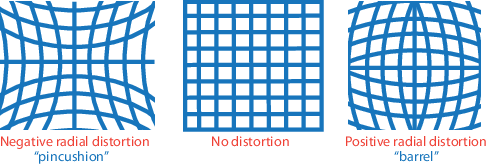
\includegraphics[width = 1\linewidth]{calibration_radial_distortion.png}
    \caption{Comparison of possible radial distortions}
    \label{fig:sec2_radial_distortion}
\end{figure}

\begin{figure}[ht]
    \centering
    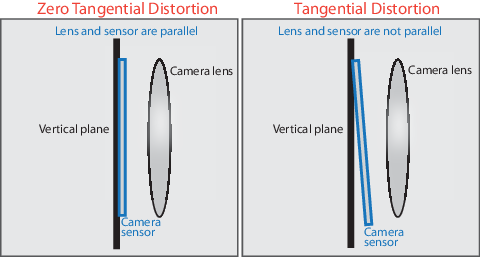
\includegraphics[width = 1\linewidth]{calibration_tangentialdistortion.png}
    \caption{Explanation for tangential distortion}
    \label{fig:sec2_tangential_distortion}
\end{figure}

Another important concept to take into account is that of camera model, which models the correspondence between points in the world and their position in image space. A common model used is the projective model (others can be used, such as perspective, affine, and orthographic models), in particular the pinhole model (Fig.\,\ref{fig:sec2_pinhole}). In this model, the mapping from world (3D) to camera (2D) is performed by tracing a ray of light from the world, through an infinitesimally small aperture (pinhole), and into the image plane. Important parameters in this model are the focal distance (distance from aperture to image plane), and image (or optical) centre (centre of the image plane), which are both intrinsic parameters. 

\begin{figure}[ht]
    \centering
    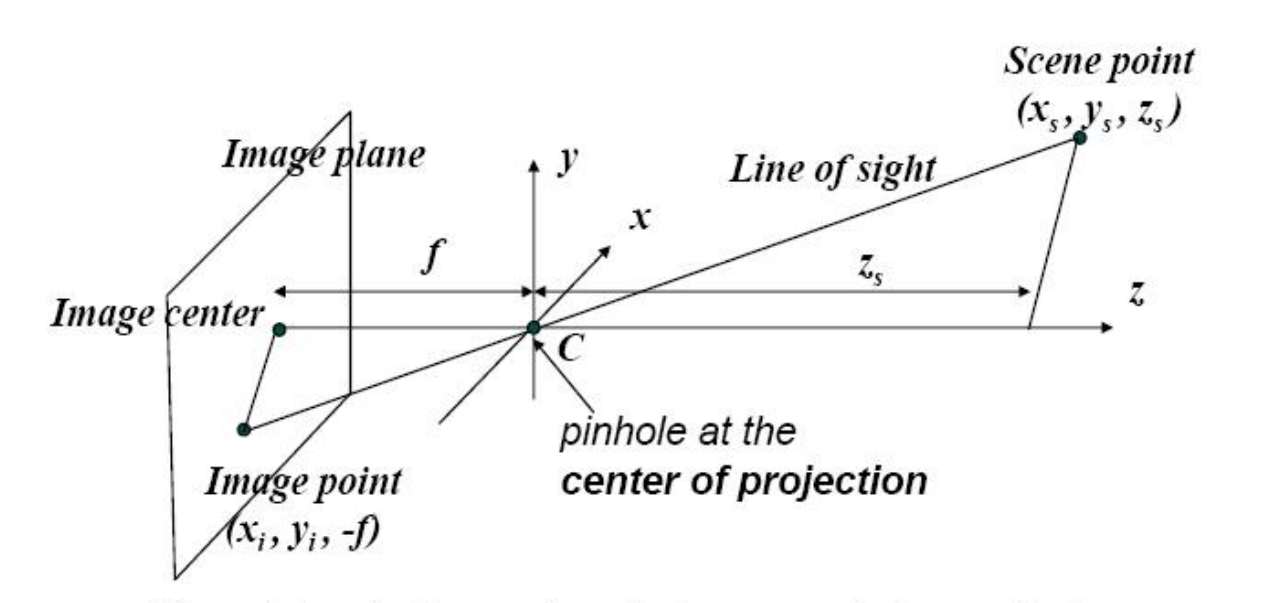
\includegraphics[width = 1\linewidth]{pinhole.png}
    \caption{Pinhole camera model}
    \label{fig:sec2_pinhole}
\end{figure}



From this model, we can derive the projective geometry, where the image plane is modelled in front of the optical centre, and the optical axis is orthogonal to the image plane. In this model, lines are projected to lines, collinear features remain collinear, and tangents and intersections are preserved, but parallel lines (in the world) eventually meet at a vanishing point, since angles are not preserved.

This geometry makes it clear that projection between world and image are given by the triangular similarity in Eq.\,\eqref{eq:sec2_projection}. 

\begin{equation}
    x=f\frac{X}{Z}, y=f\frac{Y}{Z}
    \label{eq:sec2_projection}
\end{equation}


\begin{figure}[ht]
    \centering
    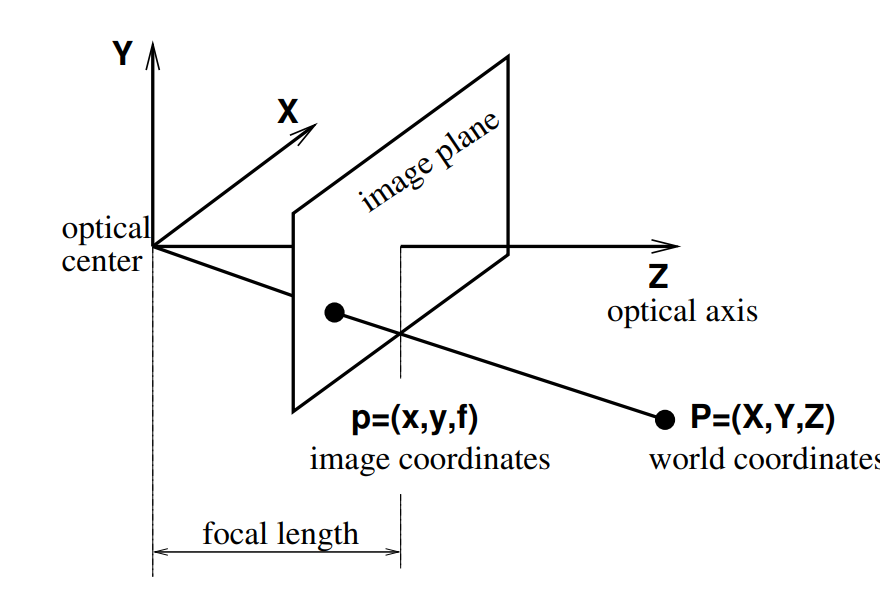
\includegraphics[width = 1\linewidth]{projective.png}
    \caption{Projective geometry}
    \label{fig:sec2_projective_geometry}
\end{figure}

The intrinsic parameters combine these properties, namely focal length ($f$), offset to the optical centre ($c_x$ and $c_y$), and skew ($s$, from non-orthogonality between optical axis and image plane), and constitute the intrinsic parameters matrix$K$, defined in Eq.\,\eqref{eq:sec2_instrinsic_matrix}. This matrix is also present in the projective matrix $P$, which relates the points in world space to their corresponding image plane position, shown in Eq.\,\eqref{eq:sec2_projective_matrix}, which is critical for computer vision.

\begin{equation}
    \label{eq:sec2_instrinsic_matrix}
    K=\begin{bmatrix}
        f_x & s & c_x\\
        0 & f_y & c_y\\
        0 & 0 & 1
    \end{bmatrix}
\end{equation}

\begin{equation}
    \label{eq:sec2_projective_matrix}
    \lambda \begin{bmatrix}
        x\\
        y\\
        1
    \end{bmatrix}=
    P
    \begin{bmatrix}
        X\\
        Y\\
        Z\\
        1
    \end{bmatrix}
    =
    \begin{bmatrix}
        K & 0
    \end{bmatrix}
    \begin{bmatrix}
        X\\
        Y\\
        Z\\
        1
    \end{bmatrix}
    =
    \begin{bmatrix}
        f_x & s & c_x & 0\\
        0 & f_y & c_y & 0\\
        0 & 0 & 1 & 0
    \end{bmatrix}
    \begin{bmatrix}
        X\\
        Y\\
        Z\\
        1
    \end{bmatrix}
\end{equation}

Assuming camera rotation and translation (extrinsic parameters, since image and world frames are not centred), the projective can be expanded to include rotation $R$ and translation $t$, and becoming completely generic, as shown in Eq.\,\eqref{eq:sec2_projective_matrix_rotation}. This is called the camera matrix.

\begin{equation}
    \label{eq:sec2_projective_matrix_rotation}
    x = K \begin{bmatrix}
        R & t
    \end{bmatrix}
    X
\end{equation}

\subsection{Camera calibration}
\label{sec:sec2_camera_calibration}

The process of finding the matrix K for a given camera is known as camera calibration. The calibration problem can be formulated as an optimization problem that matches 3D reference positions in the world, which can be either known (Direct Linear Transformation) or unknown), and the corresponding projections in the camera plane. We can assume centred image and world frames (ignore extrinsic parameters), and focus solely on intrinsic parameters, resulting in a total of 5 unknowns.

An example of calibration with known features is Direct Linear Transformation (DLT) \cite{tsai1987versatile}, in which we know the exact location of points in the 3D world and their corresponding image projection in the camera plane, and through linear equations that result from the mapping of multiple points through the camera matrix. Though this technique provides good results, a very careful setup is needed, as greater precision leads to better parameter estimation. This is not always possible, or very practical, which is why more flexible were proposed.

A popular technique is that of Zhang (\cite{zhang2000flexible}), which relies on a checkerboard planar pattern captured from at least two orientations. The high contrast of the checkerboard pattern allow for easy detection of edges and corners, as well as the plane of the checkerboard. A typical workflow consists of capturing a few images of the checkerboard under different orientations, by either moving the camera or the checkerboard, then detect feature points in the images and use a closed form solution to match 3D and 2D points, and obtain an estimation of the parameters. Afterwards, an energy optimization based on the maximum-likelihood criterion is used to fine-tune the parameters. 

\subsection{Event camera calibration}

Event cameras follow the same optical principles described in Section\,\ref{sec:sec2_camera_model}, meaning the same models are still valid, but suffer from the same distortion parameters that need to be quantified through calibration. However, due to the nature of event cameras, the techniques from Section\,\ref{sec:sec2_camera_model} cannot be applied directly. The static images of the checkerboard that are used in conventional camera calibration would just be blank images (because event cameras need movement or changes). Nevertheless, completely redesigning the last decades of computer vision calibration techniques is ill-advisable, and the technique for event cameras merely replaces the steps up until feature acquisition.

Event camera calibration is a two-stage procedure. First, a sharp image (such as the ones in Fig.\,\ref{fig:sec2_calibration_patterns}) is used, in order to focus the lenses (focus adjustment). With this procedure, the edges produced from moving the camera or the pattern should be sharp. 

\begin{figure}[ht]
	\centering
		\begin{tabular}{cc}
		   
\includegraphics[width=0.45\linewidth]{pattern.png} &
		   \hspace{1cm} 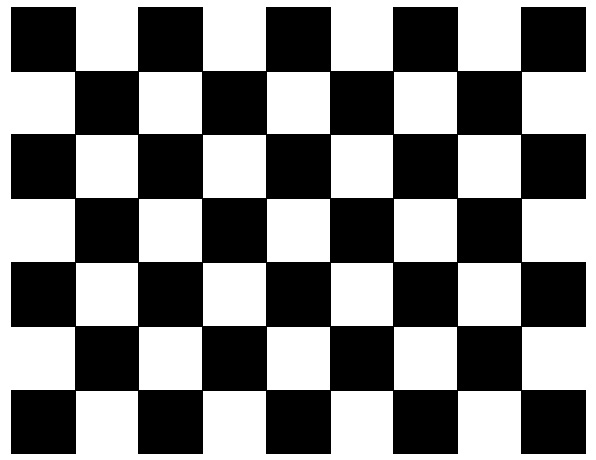
\includegraphics[width=0.45\linewidth]{chessboardpattern.jpg} \\
		   (a) & (b)  \\
		\end{tabular}
	\caption{Example images used for focus adjustment}
	\label{fig:sec2_calibration_patterns}
\end{figure}




Afterwards, a blinking LED pattern is used (Fig.\,\ref{fig:sec2_blinking}). This pattern attempts to mimic the checkerboard of conventional calibration, and the LEDs act as the corners of the checkerboard. Usually, a grid of 5x5 LEDs, spaced 5\,cm between themselves, and blinking at a frequency of 500\,Hz is used. 


\begin{figure}[ht]
	\centering
		\begin{tabular}{cc}
		   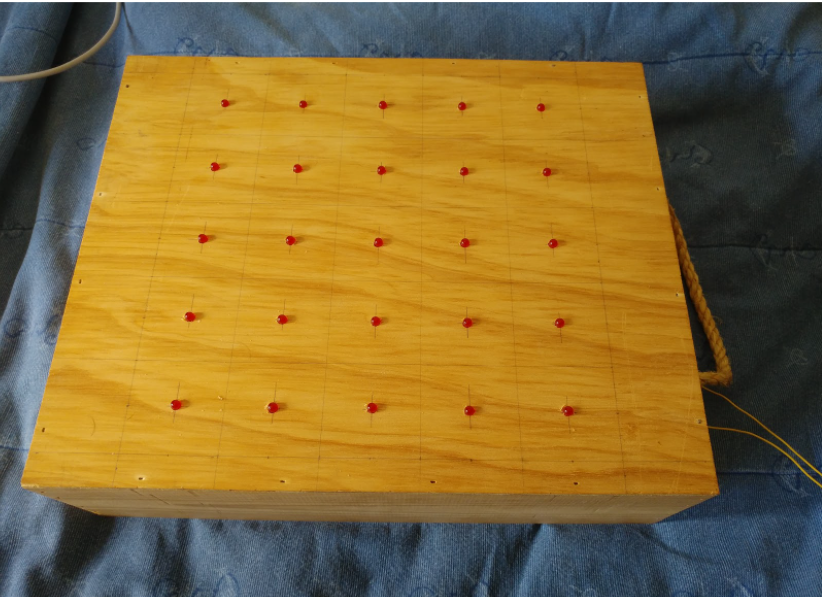
\includegraphics[width=0.45\linewidth]{box.png} &
		   \hspace{1cm} 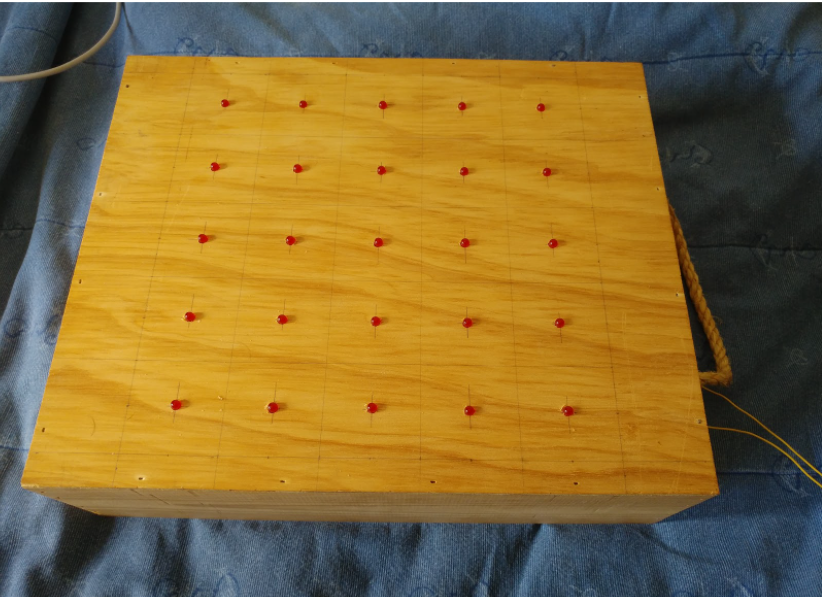
\includegraphics[width=0.45\linewidth]{box.png} \\
		   (a) & (b)  \\
		\end{tabular}
	\caption[Setup for event camera calibration]{(a) Schematic used for the connection of the LEDs, and (b) LED pattern in a rigid surface for calibration}
	\label{fig:sec2_blinking}
\end{figure}


Since the LEDs are blinking, the event camera is able to detect them and generate events, even with a still environment and camera. These events (from the blinking) are accumulated over a period of time in order to create a pseudo-frame, and blob detection is used to provide these feature to the pipeline of conventional camera calibration, which would use the corners as features. From here, the calibration pipeline is preserved.

Newer generation neuromorphic cameras combine both event and conventional camera (grayscale) acquisition. For these cameras, since the optical parameters are the same (same lens and same sensor), calibration can be performed using conventional techniques, or event camera specific techniques. The result should be the same (or similar).

% NOTA algumas imagens vieram daqui, mas nao sei mt bem como refernciar sites https://www.mathworks.com/help/vision/ug/camera-calibration.html